% begin module area-between-curves-ex5
\begin{frame}
\begin{example}%[Example 5, p. 350]
\begin{columns}
\column{.4\textwidth}
~
\psset{xunit=1.1cm, yunit=1.1cm}
\begin{pspicture}(-0.5, -1.4)(3.5,1.3)
\psframe*[linecolor=white](-0.6,-1.4)(3.6,1.3)
\tiny
\fcLabels{3.5}{1.1}
\uncover<3->{ %
\fcXTickWithLabel{0.785398163}{\alert<3>{$\frac{\pi}{4}$}}
\fcFullDot{0.785398163}{0.707106781}
} %
\fcXTickWithLabel{3.141592654}{$\pi$}

\uncover<8->{
\rput[r](-0.05,0.5){\alert<8>{$x=0$}}
\rput[l](1.64,0.5){\alert<8>{$x=\frac{\pi}{2}$}}
\pscustom*[linecolor=\fcColorAreaUnderGraph]{ %
%Function formula: \sin{}(x)
\psplot[plotpoints=1000]{0}{1.570796327}{x 57.29578 mul sin }
%Function formula: \cos{}(x)
\psplot[plotpoints=1000]{1.570796327}{0}{x 57.29578 mul cos }
} %
\rput[r](0.470796327, 0.6){$A_1$}
\rput[l](1.1, 0.6){$A_2$}
}

\uncover<5->{ %
%Function formula: \sin{}(x)
\rput[tl](2.5,0.8){$y=\sin{}(x)$}
\psplot[linecolor=\fcColorGraph, plotpoints=1000]{-0.5}{3.5}{x 57.29578 mul sin }
} %
\uncover<6->{ %
%Function formula: \cos{}(x)
\rput[rb](2.4,-1){$y=\cos{}(x)$}
\psplot[linecolor=\fcColorGraph, plotpoints=1000]{-0.5}{3.5}{x 57.29578 mul cos }
} %
\psaxes[ticks=none, labels=none]{<->}(0,0)(-0.6,-1.2)(3.5,1.2)
\end{pspicture}

%\ \ \only<handout:0| -2>{%
%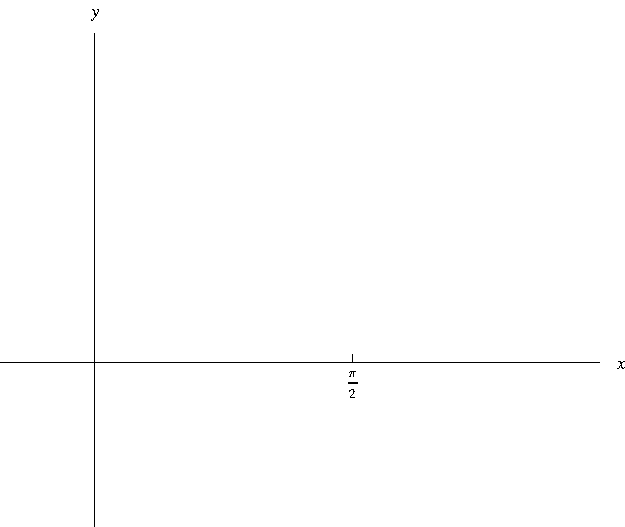
\includegraphics[height=3cm]{area-between-curves/pictures/06-01-ex5a.pdf}%
%}%
%\only<handout:0| 3-4>{%
%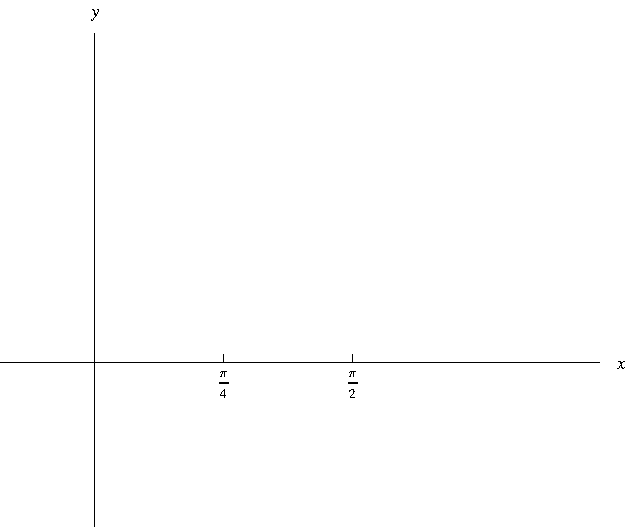
\includegraphics[height=3cm]{area-between-curves/pictures/06-01-ex5b.pdf}%
%}%
%\only<handout:0| 5>{%
%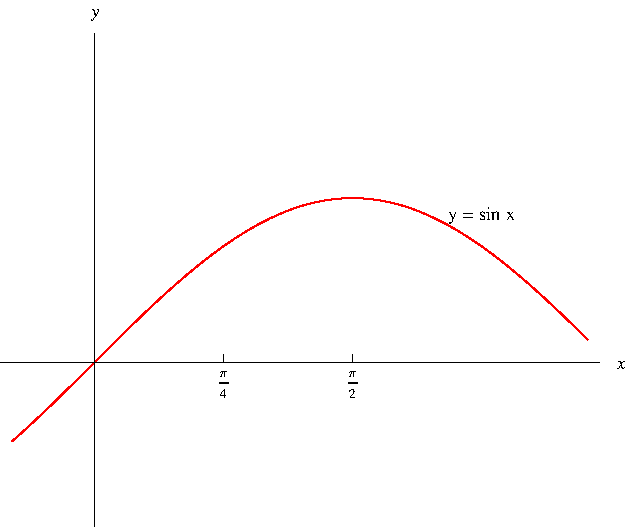
\includegraphics[height=3cm]{area-between-curves/pictures/06-01-ex5c.pdf}%
%}%
%\only<handout:0| 6-7>{%
%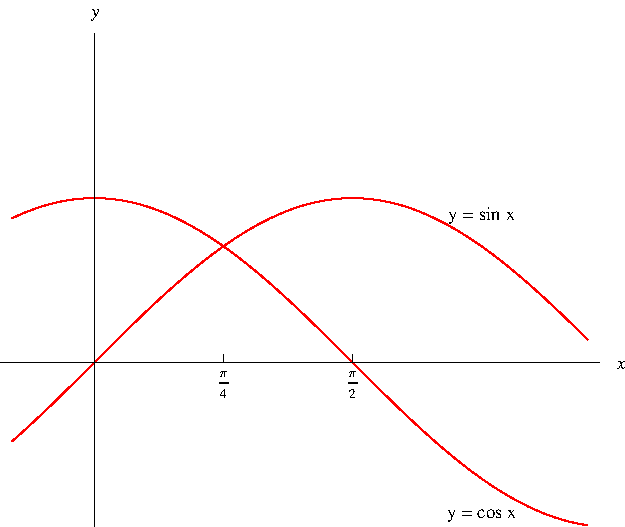
\includegraphics[height=3cm]{area-between-curves/pictures/06-01-ex5d.pdf}%
%}%
%\only<8->{%
%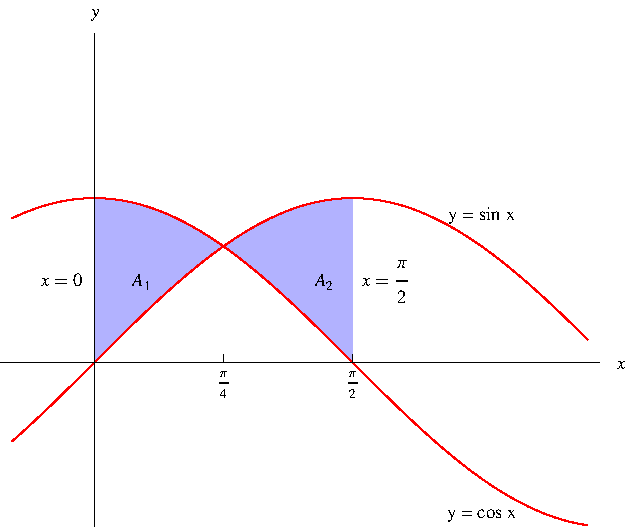
\includegraphics[height=3cm]{area-between-curves/pictures/06-01-ex5e.pdf}%
%}%
\begin{enumerate}
\item<2->  Find the point of intersection.
\item<4->  Graph the functions.
\item<7->  Identify the region.
\item<9->  Integrate.
\end{enumerate}

\column{.65\textwidth}
Find the area of the region enclosed by the curves $\alert<handout:0| 5>{y =} \alert<handout:0| 5>{\sin x}$, $\alert<handout:0| 6>{y =} \alert<handout:0| 6>{\cos x}$, $\alert<handout:0| 8>{x = 0}$ and $\alert<handout:0| 8>{x = \pi/2}$.

\uncover<3->{The only point of intersection in the interval $[0,\pi /2]$ is $(\pi /4, 1/\sqrt{2} )$.}
\abovedisplayskip=0pt
\belowdisplayskip=0pt
\abovedisplayshortskip=0pt
\belowdisplayshortskip=0pt
\begin{align*}
\uncover<8->{A} & \uncover<8->{ = A_1 + A_2} \\%
 & \uncover<9->{=}  \uncover<9->{\int_0^{\pi /4} (\cos x - \sin x )\diff x} \\
&  \qquad \uncover<9->{+ \int_{\pi /4}^{\pi /2} (\sin x - \cos x)\diff x} \\
 & \uncover<10->{=}  \uncover<10->{\left[ \sin x + \cos x \right]_0^{\pi / 4} + \left[ -\cos x - \sin x\right]_{\pi /4}^{\pi /2}}  \\
% & \uncover<11->{=}  \uncover<11->{\left[ \left( \frac{\sqrt{2}}{2} + \frac{\sqrt{2}}{2}\right) - \left( 0 + 1\right)\right] + \left[ \left( -0 - 1\right) - \left( -\frac{\sqrt{2}}{2} - \frac{\sqrt{2}}{2}\right) \right]}\\
% & \uncover<11->{=}  \uncover<11->{\left(  \frac{1}{\sqrt{2}} + \frac{1}{\sqrt{2}} - 0 - 1\right) + \left( -0 - 1 + \frac{1}{\sqrt{2}} + \frac{1}{\sqrt{2}}\right)}  \\
 & \uncover<11->{=}  \uncover<11->{2\sqrt{2} - 2.}%
\end{align*}
\end{columns}
\end{example}
\end{frame}
% end module area-between-curves-ex5
